%% ****** Start of file apstemplate.tex ****** %
%%
%%
%%   This file is part of the APS files in the REVTeX 4 distribution.
%%   Version 4.1r of REVTeX, August 2010
%%
%%
%%   Copyright (c) 2001, 2009, 2010 The American Physical Society.
%%
%%   See the REVTeX 4 README file for restrictions and more information.
%%
%
% This is a template for producing manuscripts for use with REVTEX 4.0
% Copy this file to another name and then work on that file.
% That way, you always have this original template file to use.
%
% Group addresses by affiliation; use superscriptaddress for long
% author lists, or if there are many overlapping affiliations.
% For Phys. Rev. appearance, change preprint to twocolumn.
% Choose pra, prb, prc, prd, pre, prl, prstab, prstper, or rmp for journal
%  Add 'draft' option to mark overfull boxes with black boxes
%  Add 'showpacs' option to make PACS codes appear
%  Add 'showkeys' option to make keywords appear
\documentclass[aps,pre,preprint,groupedaddress]{revtex4-1}
%\documentclass[aps,prl,preprint,superscriptaddress]{revtex4-1}
%\documentclass[aps,prl,reprint,groupedaddress]{revtex4-1}

% You should use BibTeX and apsrev.bst for references
% Choosing a journal automatically selects the correct APS
% BibTeX style file (bst file), so only uncomment the line
% below if necessary.
\bibliographystyle{apsrev4-1}
\usepackage{graphicx}
\usepackage{float}
\usepackage{amsmath}

\begin{document}

% Use the \preprint command to place your local institutional report
% number in the upper righthand corner of the title page in preprint mode.
% Multiple \preprint commands are allowed.
% Use the 'preprintnumbers' class option to override journal defaults
% to display numbers if necessary
%\preprint{}

%Title of paper
\title{\textbf{Topological Mechanics and Topological Phononic Phases}}

% repeat the \author .. \affiliation  etc. as needed
% \email, \thanks, \homepage, \altaffiliation all apply to the current
% author. Explanatory text should go in the []'s, actual e-mail
% address or url should go in the {}'s for \email and \homepage.
% Please use the appropriate macro foreach each type of information

% \affiliation command applies to all authors since the last
% \affiliation command. The \affiliation command should follow the
% other information
% \affiliation can be followed by \email, \homepage, \thanks as well.
\author{Shang Zhang}
%\email[]{Your e-mail address}
%\homepage[]{Your web page}
%\thanks{}
%\altaffiliation{}
\affiliation{Department of Physics, University of Michigan}

%Collaboration name if desired (requires use of superscriptaddress
%option in \documentclass). \noaffiliation is required (may also be
%used with the \author command).
%\collaboration can be followed by \email, \homepage, \thanks as well.
%\collaboration{}
%\noaffiliation

\date{\today}

\begin{abstract}
Topological insulators(TI), have been an important area of quantum condensed-matter research for its interesting discovery in geometric invariant in condensed matter system. This mathematics, however, appears that topological mechanisms might also exist in the acoustic spectrum of a variety of classical systems, not just electronic system as TI does. In this review, we will focus on recent study of topological mechanics and topological phononic systems, including theories and experiments, trying to provide a broad view to this new energetic area. Due to relatively simple control of mechanical systems rather than electronic systems, the topological phononic phases in classical mechanical systems have promising real-life applications. At last, we will give some general conclusions from these recent results, as well as possible future perspectives in this field.
\end{abstract}

% insert suggested PACS numbers in braces on next line
\pacs{}
% insert suggested keywords - APS authors don't need to do this
%\keywords{}

%\maketitle must follow title, authors, abstract, \pacs, and \keywords
\maketitle

% body of paper here - Use proper section commands
% References should be done using the \cite, \ref, and \label commands
\section{Introduction}
% Put \label in argument of \section for cross-referencing
%\section{\label{}}
In the past few years, with the application of ideas from the mathematical concept - topology, the mathematics describing properties that are unchangeable by smooth deformations, a new view to condensed matter system is emerging, with early discoveries in electronic system\cite{cite-key1}. People discovered interesting phenomenology of electrons in TIs, which are a kind of material with non-trivial topological order that behaves as an insulator in its interior but whose surface contains conducting states, meaning that electrons can only move along the surface of the material\cite{cite-key1,cite-key2,cite-key3}.

Following an explosion of studying in topological phases in hard condensed matter, this topological approach has recently been used from the quantum realm of electrons to the world of classical mechanical systems.  Electronic TIs have inspired the design of new topological mechanical systems that could lead to new design principles for metamaterials\cite{huber2016topological}. In this review, we will try to establish the connections between topological electrons systems to classical mechanical systems based on recent research work, as well as perspectives in this field.

\subsection{Analogy between Quantum and Newton's Mechanics}

At first sight, electronic systems described by quantum mechanics seem totally different to mechanical modes described by Newton's equations of motion, but it is not always the case.

In 1985, it was discovered that similar geometric phases to Berry's phase \cite{cite-key5} occurred in classical systems with single or few mechanical modes \cite{cite-key9}, which illustrates the appearance of geometric phases in classical systems.

From the inspiration of development of TI, it was discovered that bulk and boundary states of phononic systems can show similar properties seen in TI\cite{cite-key11,cite-key12}. These results confirmed the guess that there's some analogy between quantum and newton's mechanics that can introduce the same topological properties in electronic and phononic systems.

To illustrate the analogy between quantum and Newton's mechanics, we consider the equation of motions in a network of coupled simple harmonic oscillators,
\begin{align}
\ddot{x}_i &= -D_{ij}x_j+A_{ij}\dot{x}_j
\label{eq1}
\end{align}

Where the dynamical matrix $D$ is real and positive definite, and $A$ is a skew symmetric matrix, describing the coupling between velocities and positions. Then \cite{susstrunk2016classification} one can rewrite equation (\ref{eq1}) to,

\begin{align}
i\frac{\partial}{\partial t}
\begin{pmatrix}
\sqrt{D}^{T}x\\
i\dot{x}
\end{pmatrix}
&=
\begin{pmatrix}
0 & \sqrt{D}^{T}\\
\sqrt{D} & iA
\end{pmatrix}
\begin{pmatrix}
\sqrt{D}^{T}x\\
i\dot{x}
\end{pmatrix}
\label{eq2}
\end{align}

Equation (\ref{eq2}) transfers Newton's equations into Hermitian eigenvalue equations, in similar form to Schrodinger equation. Solving for phononic frequency $\omega$ to get the mechanical modes, there is one important property: Because of the real, positive definite matrix $D$ and skew symmetric matrix $A$, any solutions of $\omega$ for equation (\ref{eq1}) will have a corresponding symmetric solution $-\omega$.

Kane and Lubensky used a similar way to illustrate this symmetry for classical spring network\cite{cite-key10}. They borrowed the concept of supersymmetry to illustrate this property and construct Hamiltonian with dynamical matrix $D = QQ^T$ and its supersymmetric partner $\tilde{D} = Q^TQ$,

\begin{align}
\mathcal{H} = 
\begin{pmatrix}
0 & Q\\
Q^T & 0
\end{pmatrix};
&\mathcal{H}^2 = 
\begin{pmatrix}
QQ^T & 0\\
0 & Q^TQ
\end{pmatrix}
\label{eq3}
\end{align}

Both of these two representations from equation (\ref{eq2}) and equation (\ref{eq3}) show that there is an intrinsic 'particle-hole' symmetry in classical spring networks, and this symmetry can be analyzed in the framework of topological band theory\cite{cite-key2}. As a result, this 'supersymmetry' is the origin of topological phenomena for mechanical modes.

\subsection{Present Topological Mechanical System}

Based on the symmetric similarity between topological band description in electronic systems and Newton's mechanics in classical spring networks, there are three approaches to present topological boundary modes in classical mechanical systems:
\begin{itemize}
\item Directly utilize the intrinsic 'particle-hole' symmetry
\item Engineer a topological dynamical matrix $D$
\item Engineer matrix $A$ to provide broken time-reversal symmetry
\end{itemize}

In the first case, topological boundary modes appear in the gap around zero frequency, with the zero-frequency 'floppy modes' localized on the boundaries. The topological boundary modes in isostatic lattices, which are on the onset of mechanical instability, appear to be topological protected, similar to the protected electronic boundary modes.

For the latter two cases, the stable topological boundary phases appear at non-zero frequencies. Engineering the dynamical matrix $D$ and matrix $A$ in proper way is the key to present topological mechanical system.

\section{Zero-frequency}

Based on the intrinsic 'particle-hole' symmetry, Kane and Lubensky studied the topological edge states in isostatic lattices, which are on the onset of mechanical instability. They've developed a general theory of topological phases on isostatic lattices, and illustrated the connection between electronic topological band theory to topological boundary zero modes\cite{cite-key10}. Then there are some experimental results based on their theoretical prediction\cite{cite-key19,cite-key20,cite-key21,cite-key22}.

\subsection{A One-Dimensional Model}

We will introduce a one-dimensional model as an simple example to illustrate the topological boundary modes in isostatic lattices\cite{lubensky2015phonons}.

This model, as described in figure \ref{fig1}, has same phonon spectrum to one-dimensional Su-Schrieffer-Heeger model\cite{su1979solitons}, which is a well-studied model for the electronic excitations of polyacetylene($(CH_2)_n$). It consists of rigid rods with the length of $r$, rotating freely about the fixed axis, and the axises are separated by length $a$. The end of these neighbored rods are connected by harmonic springs. $\bar{\theta}$ is the angle of the rotated rod with the upward or downward norms, with tilt to the right $\bar{\theta} > 0$, tilt to the left $\bar{\theta} < 0$. Then each rod $s$ has one degree of freedom, $\theta_s = \bar{\theta} - \delta \theta_s$.

\begin{figure}[h]
\centering
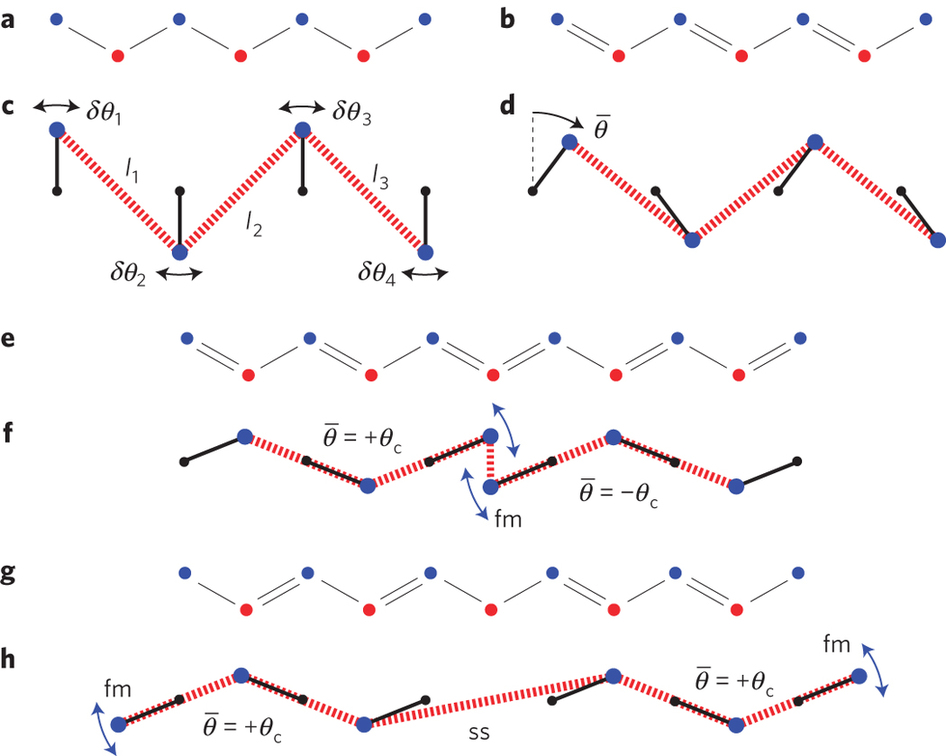
\includegraphics[scale=0.4]{nphys2835-f1.jpg}
\caption{One Dimensional Model for Topological Phonon}
\label{fig1}
\end{figure}

In linearized limit, consider the compatibility matrix $C$ with components $C_{\beta s}$, the stretch in spring $\beta$ with rotations at rod $s$ is given as $\delta l_{\beta} = \sum_{s} C_{\beta s} \delta \theta_{s}$.

Since one rod is only connected to its neighbored springs, the compatibility matrix at rest angle $\bar{\theta}$ can be given as,
\begin{align}
C_{\beta s}(\bar{\theta}) &= c_1(\bar{\theta}) \delta_{s,\beta} - c_2(\bar{\theta})\delta_{\beta, s+1}
\end{align}

Solve for $c_1, c_2$ in the spring system, we can get,
\begin{align}
c_{1(2)} &= \displaystyle \frac{(a \pm 2r \sin{\theta})r\cos{\theta}}{\sqrt{a^2+4r^2\cos^2{\bar{\theta}}}}
\end{align}

Thus $|c_1| > |c_2|$, for all $0 < \bar{\theta} < \pi$ and $|c_1| < |c_2|$ for all $-\pi < \bar{\theta} < 0$. Then the Fourier transform of $C_{s\beta}$ is,
\begin{align}
C(q) &= c_1 - e^{iqa}c_2
\label{eq6.4}
\end{align}

and the bulk phonon modes have frequency,
\begin{align}
\omega(q) = \pm |C(q)| = \pm \sqrt{(c_1-c_2)^2+4c_1c_2\sin^2{(qa/2)}}
\end{align}

So for $c_1 = c_2$, there is a bulk zero mode at $q=0$. This is a trivial mode for all the bases of rods anchored. For other values of $\bar{\theta}$, solve for zero modes $\omega(q) = 0$, we can get imaginary $q$ for zero mode, introducing the decay of surface zero modes into the bulk.

\subsection{Winding Number}

Still look at the one-dimensional model, the compatibility matrix $C(q) \equiv |C(q)|^{i \phi}$ in the complex plane will be mapped in the Brillouin zone $(-\pi/a<q \leq \pi/a)$ as closed path in the zone $[q \rightarrow q+(2\pi/a)]$. Then the $C(q)$ can characterize an integer,
\begin{align}
n = \frac{1}{2\pi} \int_0^{2\pi} \mathrm{d}\phi = \frac{1}{2\pi} \int_0^{2\pi} \mathrm{d}q \frac{\mathrm{d}}{\mathrm{d}q} {Im \ln \det C(q)}
\end{align}

Then for the $C(q)$ in equation (\ref{eq6.4}), $n = +1$ or $0$. $n=0$ is for the case that the path in complex plane doesn't enclose the origin while $n=+1$ if does. The winding number is a topological invariant to $\bar{\theta}$ and will only change when passing the critical angles $\bar{\theta} = 0$ or $\bar{\theta} = \pi$. 

Similar to the winding number for $C(q)$, one can also define the winding number for $Q(q)$. Then Kane and Lubensky gave a more general form of winding number for topological lattices which are two-dimensional system as,
\begin{align}
n_i = \frac{1}{2\pi} \oint_{C_i} \mathrm{d}\mathbf{q} \cdot Tr[{\mathbf{Q}(\mathbf{q})^{-1}}\nabla_{\mathbf{q}}{\mathbf{Q}(\mathbf{q})}] = 
\frac{1}{2\pi} \oint_{C_i} \mathrm{d}\mathbf{q} \cdot \nabla_{\mathbf{q}}{\phi(\mathbf{q})}
\end{align}
where $\phi(\mathbf{q})$ is the phase of $\det \mathbf{Q}(\mathbf{q})$ $(\mathbf{Q}(\mathbf{q}) = |\mathbf{Q}(\mathbf{q})|^{i \phi(\mathbf{q})})$. And $C_i$ is a closed path of the BZ with the connecting of $\mathbf{q}$ and $\mathbf{q}+\mathbf{B}_i$, where $\mathbf{B}_i$ is a primitive reciprocal vector satisfying $\mathbf{a}_i\mathbf{B}_j = 2\pi \delta_{ij}$.

Then with the winding number, the topological modes of isostatic Maxwell lattices are divided into two behaviors. A positive winding number is related to the zero modes which are free to move. While a negative winding number is related to a localized state of self stress, where there're no forces between elements even though there are the finite stresses on between.

\subsection{Experimental Applications}

Recent experimental implementations are applied onto topological edge modes of isostatic lattices.

The one-dimensional topological phononic system has been implemented and confirmed the predicted floppy modes\cite{cite-key19}. And moreover, nonlinear effects in this 1-D model is shown to transport floppy modes trough the bulk\cite{cite-key20}, which is beyond the theory straightforwardly introduced by topological band theory.

Besides the boundary floppy modes, localized states of self-stress are also studied\cite{cite-key21}. Then application to Origami and Kirigami has also been done, showing topological phenomena in these systems\cite{cite-key22}.

\section{Finite-frequency}

To artificially present topological edge modes at finite frequency, there are three main challenges compared to electronic topological systems.
\begin{itemize}
\item The breaking of time-reversal symmetry in acoustic systems needs nonreciprocal sound transmission, which are not easy to get.
\item Time-reversal operator should be squared to $-1$, which is pretty easy to have in spin $-1/2$ particles but not for phonon.
\item Phonon are relatively easy to be produced discretely, while practical materials are usually continuous, which is not quite applicable to produce continuous topological phononic system.
\end{itemize}

\subsection{Discrete Oscillator Implementation}

Several recent experiments succeed in solving the first two problems by designing with some new-developed technology. These breakthroughs provide clever ways to implement discrete finite-frequency topological phononic system, which are quite inspiring.

A set of two-dimensional hanging gyroscopes was designed with the help of an efficient way to produce non-reciprocal sounds, leading to strict unidirectional transport in certain frequency range, with effective time-reversal symmetry breaking\cite{cite-key29}. Besides this system, the apparent spin $-1/2$ effects are implemented classically with coupled pendula network, appearing a good analogy to quantum spin Hall effect\cite{cite-key30}.

However, both of these examples given above are implemented in discrete local phononic sources (like pendula and gyroscopes), which is an obvious shortage urging researchers to study the continuous systems.

\subsection{Continuous Systems}

Some relative simple topological phononic systems have been implemented, providing good efforts to better handle continuous systems, which should have large applicable possibilities to real life.

An experiment based on the continuous one-dimensional SSH model has observed localized modes\cite{cite-key31}. And the topological band structures of two-dimensional case have also been measured in metallic cylinders of engineered honeycomb lattice\cite{he2015acoustic}.

\section{Conclusion and Perspective}

\subsection{Conclusion}

With recent prosperity in the study of topological electronic systems, the topological view to classical mechanical systems seems to be natural and has solid theoretical reference. However, the great differences between mechanical modes to electronic modes are still producing great challenges for the study of topological mechanics.

A general theory of topological phases of isostatic lattices is given\cite{cite-key10}, and there're also a large amount of experiments trying to build a good bridge between phononic and electronic modes\cite{cite-key19,cite-key20,cite-key21,cite-key22,cite-key29,cite-key30,cite-key31,he2015acoustic}. Compared to the topological phase properties in electronic system, they come from very similar phenomenology. 

As a result, the topological boundary modes are an elegant consequence of a widely-used mathematical structure, in topological electronic systems as well as mechanical modes of classical systems.

\subsection{Perspective}

Classical mechanical systems make it convenient to put the topological states into real-life applications rather than electronic system, which is one of the most exciting potential for topological mechanics. Many new challenging problems are still unsolved on the study of topological mechanical systems. This field is very promising.

In particular, for finite frequency case of topological mechanics, continuous systems still remain challenging to handle. More general theories and setups to control continuous topological mechanical systems are needed and interesting.

Since current theory and implementations are restricted to one and two dimensional systems, it would be very useful to further the study of 3-dimensional topological mechanical system.

Besides, nonlinear effects of topological mechanical systems might provide some new and surprising results beyond the straightforward linear topological phononic theory.

% If in two-column mode, this environment will change to single-column
% format so that long equations can be displayed. Use
% sparingly.
%\begin{widetext}
% put long equation here
%\end{widetext}

% figures should be put into the text as floats.
% Use the graphics or graphicx packages (distributed with LaTeX2e)
% and the \includegraphics macro defined in those packages.
% See the LaTeX Graphics Companion by Michel Goosens, Sebastian Rahtz,
% and Frank Mittelbach for instance.
%
% Here is an example of the general form of a figure:
% Fill in the caption in the braces of the \caption{} command. Put the label
% that you will use with \ref{} command in the braces of the \label{} command.
% Use the figure* environment if the figure should span across the
% entire page. There is no need to do explicit centering.

% Surround figure environment with turnpage environment for landscape
% figure
% \begin{turnpage}
% \begin{figure}
% \includegraphics{}%
% \caption{\label{}}
% \end{figure}
% \end{turnpage}

% tables should appear as floats within the text
%
% Here is an example of the general form of a table:
% Fill in the caption in the braces of the \caption{} command. Put the label
% that you will use with \ref{} command in the braces of the \label{} command.
% Insert the column specifiers (l, r, c, d, etc.) in the empty braces of the
% \begin{tabular}{} command.
% The ruledtabular enviroment adds doubled rules to table and sets a
% reasonable default table settings.
% Use the table* environment to get a full-width table in two-column
% Add \usepackage{longtable} and the longtable (or longtable*}
% environment for nicely formatted long tables. Or use the the [H]
% placement option to break a long table (with less control than 
% in longtable).
% \begin{table}%[H] add [H] placement to break table across pages
% \caption{\label{}}
% \begin{ruledtabular}
% \begin{tabular}{}
% Lines of table here ending with \\
% \end{tabular}
% \end{ruledtabular}
% \end{table}

% Surround table environment with turnpage environment for landscape
% table
% \begin{turnpage}
% \begin{table}
% \caption{\label{}}
% \begin{ruledtabular}
% \begin{tabular}{}
% \end{tabular}
% \end{ruledtabular}
% \end{table}
% \end{turnpage}

% Specify following sections are appendices. Use \appendix* if there
% only one appendix.
%\appendix
%\section{}

% If you have acknowledgments, this puts in the proper section head.
%\begin{acknowledgments}
% put your acknowledgments here.
%\end{acknowledgments}

% Create the reference section using BibTeX:
\bibliography{TermPaper}

\end{document}
%
% ****** End of file apstemplate.tex ******

